% Versión para diapositiva (plantilla Semana ICG 2026): tamaño real 1:1, texto de 24 pt.
% Insertar en PowerPoint al 100 % (cabe en el área de contenido de 35 x 11,6 cm).
\documentclass[border=2pt]{standalone}
\usepackage{iftex}
\ifPDFTeX
  \usepackage[utf8]{inputenc}
  \usepackage[T1]{fontenc}
  \usepackage[sfdefault]{carlito}
\else
  \usepackage{fontspec}
  \setmainfont{Carlito}[Extension=.ttf, UprightFont=*-Regular, BoldFont=*-Bold,
    ItalicFont=*-Italic, BoldItalicFont=*-BoldItalic]
\fi
\usepackage{tikz}
\usetikzlibrary{arrows.meta, positioning}

\definecolor{tinta}{HTML}{1B2A3A}
\definecolor{azul}{HTML}{1D5F83}
\definecolor{azulosc}{HTML}{164A66}
\definecolor{verde}{HTML}{5E8C45}
\definecolor{grisazul}{HTML}{7F9BB8}

\begin{document}
\fontsize{24}{29}\selectfont
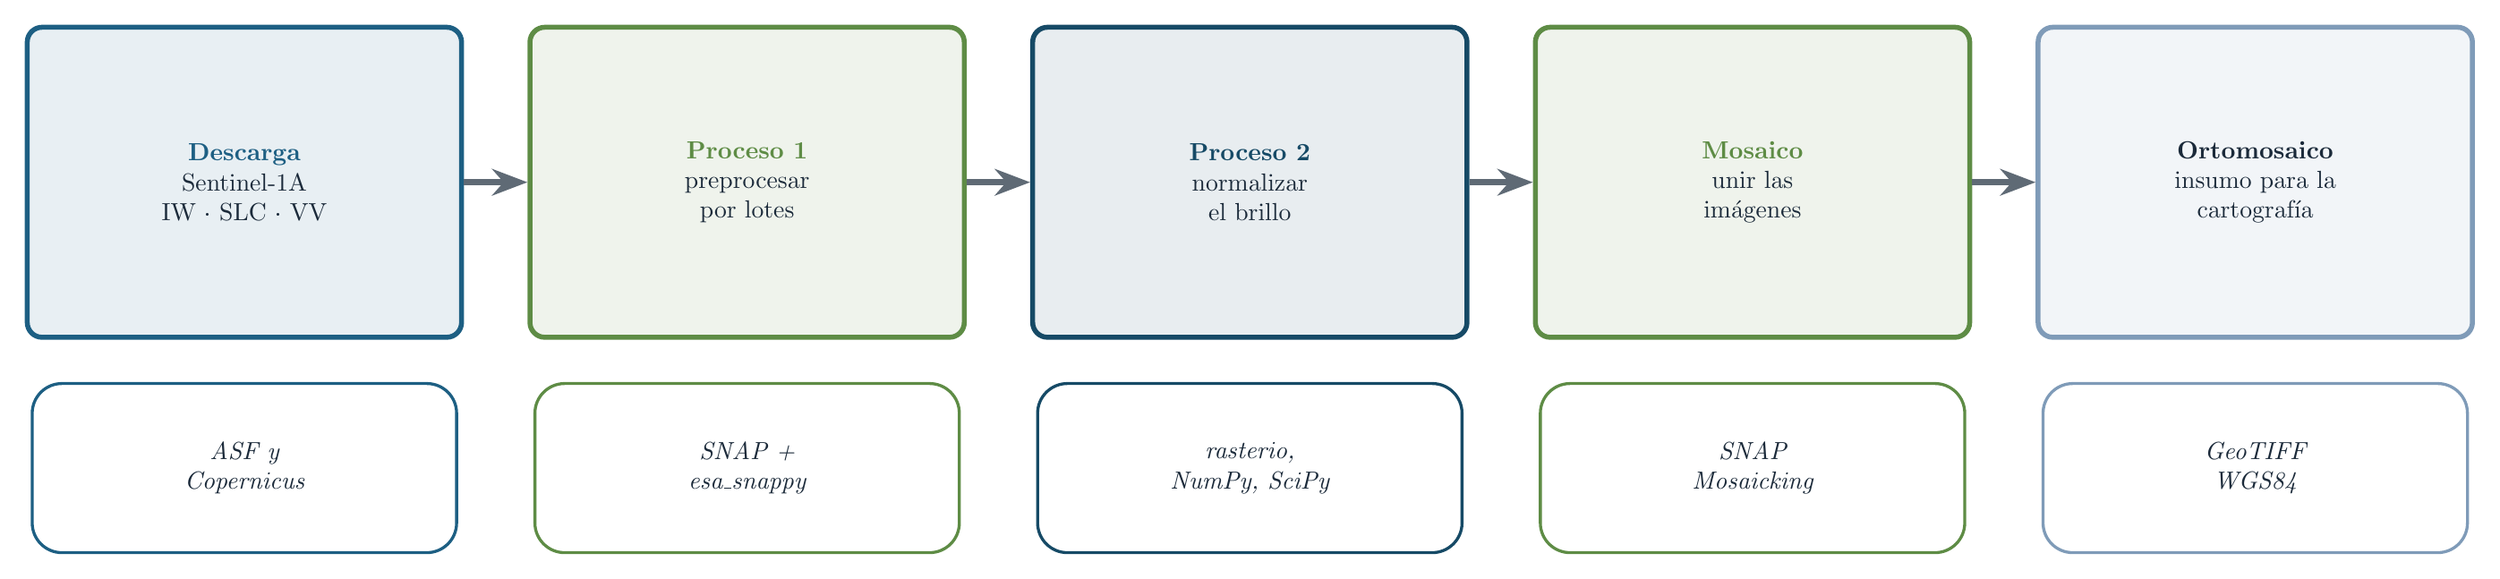
\begin{tikzpicture}[
  >=Stealth,
  fase/.style={rectangle, rounded corners=6pt, draw=#1, line width=2pt,
               fill=#1!10, text width=5.6cm, minimum height=4.4cm,
               align=flush center, text=tinta, inner sep=8pt},
  herr/.style={rectangle, rounded corners=12pt, draw=#1, line width=1.2pt,
               fill=white, text width=5.6cm, minimum height=2.4cm,
               align=flush center, text=tinta, font=\itshape, inner sep=6pt},
  flecha/.style={->, line width=2.5pt, draw=tinta!70}
]
\node[fase=azul] (f1) {\textbf{\color{azul}Descarga}\\ Sentinel-1A\\ IW · SLC · VV};
\node[fase=verde, right=9mm of f1] (f2) {\textbf{\color{verde}Proceso 1}\\ preprocesar\\ por lotes};
\node[fase=azulosc, right=9mm of f2] (f3) {\textbf{\color{azulosc}Proceso 2}\\ normalizar\\ el brillo};
\node[fase=verde, right=9mm of f3] (f4) {\textbf{\color{verde}Mosaico}\\ unir las\\ imágenes};
\node[fase=grisazul, right=9mm of f4] (f5) {\textbf{\color{tinta}Ortomosaico}\\ insumo para la\\ cartografía};

\foreach \a/\b in {f1/f2, f2/f3, f3/f4, f4/f5}
  \draw[flecha] (\a.east) -- (\b.west);

\node[herr=azul,     below=6mm of f1] {ASF y\\ Copernicus};
\node[herr=verde,    below=6mm of f2] {SNAP +\\ esa\_snappy};
\node[herr=azulosc,  below=6mm of f3] {rasterio,\\ NumPy, SciPy};
\node[herr=verde,    below=6mm of f4] {SNAP\\ Mosaicking};
\node[herr=grisazul, below=6mm of f5] {GeoTIFF\\ WGS84};
\end{tikzpicture}
\end{document}
